    \section{Триангуляция и картинная галерея}

    \begin{frame}{Лемма о триангуляции}

    \vspace{2mm}
    \begin{lm}[О триангуляции]\hypertarget{trianglemm}{}

        Всякий многоугольник можно диагоналями разбить на треугольники, причем полученный граф красится в 3 цвета.

    \end{lm}

    \begin{proof}\let\qed\relax
        Индукция по числу вершин.\\

        \textbf{База:} $n = 3$.\\
        \textbf{Переход:} Находим вершину с  углом $<180^{\circ}$.\\

        \begin{itemize}

            \item Отрезок между соседними  вершинами лежит в многоугольнике:\\
            Отрезаем вершину, красим по индукции, возвращаем, красим в свободный цвет.

        \end{itemize}

    \end{proof}

    \end{frame}

    \begin{frame}{Лемма о триангуляции: доказательство}

    \vspace{2mm}

    \begin{proof}\let\qed\relax

        \begin{center}
        \begin{tikzpicture}[scale = 0.25]
        \begin{scope}
        \coordinate (a) at (0,0); \coordinate (b) at (-3,1); \coordinate (c) at (-2, 5); \coordinate (d) at (1, 7); \coordinate (e) at (4, 4); \coordinate (f) at (7, 6); \coordinate (g) at (8, 1);
        \draw[fill1, fill = fill1] (a) circle (0.1);\draw[fill4, fill = fill4] (b) circle (0.1); \draw[fill4, fill = fill4] (c) circle (0.1); \draw[fill4, fill = fill4] (d) circle (0.1); \draw[fill4, fill = fill4] (e) circle (0.1); \draw[fill4, fill = fill4] (f) circle (0.1); \draw[fill4, fill = fill4] (g) circle (0.1);
        \draw[fill4, thick] (c)--(d)--(e)--(f)--(g)--(a);
        \draw pic[draw, thick, fill1, angle radius=0.2cm, shift={(6mm,1mm)}] {angle=a--b--c};
        \draw[fill1, thick, dashed] (b)--(c);
        \draw[fill1, thick, dashed] (a)--(b);
        \draw[fill1, thick, dashed] (a)--(c);
        \end{scope}
        \begin{scope}[xshift = 15cm]
        \coordinate (a) at (0,0); \coordinate (b) at (-3,1); \coordinate (c) at (-2, 5); \coordinate (d) at (1, 7); \coordinate (e) at (4, 4); \coordinate (f) at (7, 6); \coordinate (g) at (8, 1);
        \draw[fill4, fill = fill4] (a) circle (0.1);\draw[fill4, fill = fill4] (b) circle (0.1); \draw[fill4, fill = fill4] (c) circle (0.1); \draw[fill4, fill = fill4] (d) circle (0.1); \draw[fill4, fill = fill4] (e) circle (0.1); \draw[fill4, fill = fill4] (f) circle (0.1); \draw[fill4, fill = fill4] (g) circle (0.1);
        \draw[fill4, thick] (a)--(c)--(d)--(e)--(f)--(g)--cycle;
        \draw pic[draw,  thick, fill1, angle radius=0.2cm, shift={(6mm,1mm)}] {angle=a--b--c};
        \draw[fill4, thick] (a)--(d);
        \draw[fill4, thick] (a)--(e);
        \draw[fill4, thick] (e)--(g);
        \draw[fill1, dashed, thick] (b)--(c);
        \draw[fill1, dashed, thick] (a)--(b);
        \end{scope}
        \end{tikzpicture}
        \end{center} \vspace{-7mm}

        \begin{itemize}
        \item Отрезок между соседними  вершинами не лежит в многоугольнике:

        \begin{center}
        \begin{tikzpicture}[scale = 0.25]
        \begin{scope}
        \coordinate (a) at (0,0); \coordinate (b) at (3,6); \coordinate (c) at (8, 7); \coordinate (d) at (3, 2); \coordinate (e) at (9, 0); \coordinate (f) at (-2, 7); \coordinate (g) at (7, -2);
        \draw[fill1, fill = fill1] (a) circle (0.1);\draw[fill4, fill = fill4] (b) circle (0.1); \draw[fill4, fill = fill4] (c) circle (0.1); \draw[fill4, fill = fill4] (d) circle (0.1); \draw[fill4, fill = fill4] (e) circle (0.1);
        \draw[fill4, thick] (a)--(b)--(c)--(d)--(e)--cycle;
        \draw[fill1, thick] (b)--(e);
        \draw[fill1, thick] (f)--(g);
        \draw pic[draw,  thick, fill1, angle radius=0.35cm, shift={(6mm,1mm)}] {angle=e--a--b};
        \end{scope}
        \begin{scope}[xshift = 15cm]
        \coordinate (a) at (0,0); \coordinate (b) at (3,7); \coordinate (c) at (8, 7); \coordinate (d) at (3, 2); \coordinate (e) at (11, 0); \coordinate (f) at (-3, 7);
        \draw[fill1, fill = fill1] (a) circle (0.1);\draw[fill4, fill = fill4] (b) circle (0.1); \draw[fill4, fill = fill4] (c) circle (0.1); \draw[fill4, fill = fill4] (d) circle (0.1); \draw[fill4, fill = fill4] (e) circle (0.1);
        \draw[fill4, thick] (a)--(b)--(c)--(d)--(e)--cycle;
        \draw[fill1, thick] (a)--(d);
        \draw[fill4, thick] (b)--(d);
        \draw[fill4, thick] (b)--(d);
        \end{scope}
        \end{tikzpicture}
        \end{center}

    \end{itemize}

    \end{proof}

    \end{frame}

    \subsection{Задача о картинной галерее}

    \begin{frame}{Задача о картинной галерее}

        \begin{task}

            Дана картинная галерея, план которой~--- многоугольник без самопересечений. Какое минимальное число охранников нужно поставить в точках галереи, чтоб
            они просматривали каждую точку?

        \end{task}

    \end{frame}

    \begin{frame}{Задача о картинной галерее: иллюстрация}
\begin{center}
  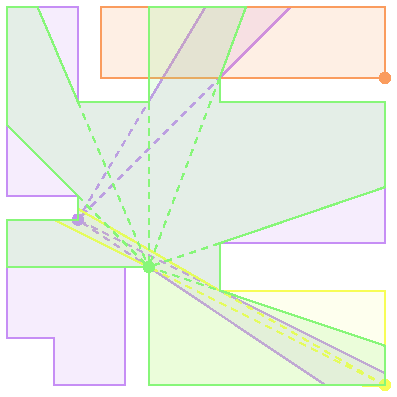
\includegraphics[height=0.84\textheight]{svg/pictGallery}
\end{center}
    \end{frame}

    \begin{frame}{Задача о картинной галерее}
        
        \vspace{2mm}
        \begin{thm}[Хватал]
		Для произвольного $n$-угольника
		достаточно $\lfloor \frac{n}{3} \rfloor$ охранников,\\
		поставленных во внутренних точках, чтобы охранникам\\
		были видны все внутренние точки $n$-угольника.
        \end{thm}

        \begin{block}{Доказательство}
		По \hyperlink{trianglemm}{лемме} строим разбиение
		галереи на треугольники,\\
		вершины раскрашиваются в три цвета. Из этих цветов\\
		выбираем тот, который встречается \emph{не чаще других}.\\
		Ставим охранников в вершины, окрашенные этим цветом.
        \end{block}
    \end{frame}
